\documentclass{article}

\date{16 décembre 2023}
\usepackage[nb-sem=12, auteurs={Kylian Boyet, Hugo Vangilluwen, George Ober (relecture)}]{../kholles}

\begin{document}
\maketitle

\begin{question_kholle}
  [Soient $a \in \K$ et $v \in \K^\N$ où \K peut être \C ou \R.
    L'ensemble des solutions de l'équation $\forall n \in \N, u_{n+1} = au_{n} + v_{n}$
    est la droite affine :
    \begin{equation}
      \left\{ w + \lambda \left( a^n \right) _{n \in \N} \mid \lambda \in \K \right\}
    \end{equation}
  ]
  {Résolution d'une relation de récurrence linéaire d'ordre 1 à coefficients constants et avec second membre}

  Posons $w$ la suite définie par $$
    \left\{ \begin{array}{ll}
      w_{0} = 1 \\
      \forall n \in \N, w_{n+1} = aw_{n} + v_{n}
    \end{array}\right.
  $$
  $w$ est "évidemment solution de particulière de l'équation"

  Maintenant que nous disposons d'une solution particulière, et ayant observé que l'équation est linéaire, mettons en œuvre l'artillerie classique pour exprimer l'ensemble des solutions par l'habituelle technique.


  \begin{align*}
    \forall n \in \N, u_{n+1} = au_{n} + v_{n} & \iff \forall n \in \N, u_{n+1} - au_{n} = v_{n}                                                         \\
                                                       & \iff \forall n \in \N, u_{n+1} - au_{n} = w_{n+1} - aw_{n}                                              \\
                                                       & \iff \forall n \in \N, (u-w)_{n+1} = a(u-w)_{n}                                                         \\
                                                       & \iff u-w \in \text{Vect}\left\{ \left( a^n \right) _{n \in \N} \right\}                                 \\
                                                       & \iff \exists \lambda \in \K : u-w = \lambda \left( a^{n} \right) _{n \in \N}                    \\
                                                       & \iff \exists \lambda \in \K : \forall n \in \N, u_{n} = w_{n} + \lambda a^n                     \\
                                                       & \iff  u \in \left\{ \left( w_{n} + \lambda a^n \right) _{n \in \N} \mid \lambda \in \K \right\}
  \end{align*}

\end{question_kholle}

\begin{question_kholle}
  [Soient $(a,b) \in \C^2$.
    L'ensemble des solutions $S_H$ de l'équation d'inconnue $u \in \C^\N$
    \begin{equation}
      \forall n \in \N, u_{n+2} = a u_{n+1} + b u_n
    \end{equation}
    est le plan vectoriel $\text{Vect}\{ \left(r_1^n\right)_{n\in\N}, \left(r_2^n\right)_{n\in\N} \}$ où $r_1$ et $r_2$ sont les racines de l'équation caractéristique ($r^2 = ar + b$) quand $\Delta \neq 0$.]
  {Résolution d'une relation de récurrence linéaire homogène d'ordre 2 à coefficients constants dans \C lorsque l'équation caractéristique possède un discriminant non nul}

  Soient $(a,b) \in \C^2$ fq.

  \underline{Lemme} Soit $r \in \C$. $\left(r^n\right)_{n\in\N}$ est solution de l'équation de récurrence si et seulement si $r^2 = ar + b$.
  \begin{equation*}
    \begin{aligned}
      (r^n)_{n\in\N} \text{ est solution }
      \iff \forall n \in \N, r^{n+2}                                                    & = a r^{n+1} + b r^n \\
      \iff \forall n \in \N, r^{n} \left( r^2 - a r - b \right)                         & = 0                 \\
      \underbrace{\iff}_{\text{ En particularisant pour } n \leftarrow 0} r^2 - a r - b & = 0                 \\
      \iff r^2                                                                          & = a r + b
    \end{aligned}
  \end{equation*}

  Considérons le cas où l'équation $r^2 = ar + b$ admet deux racines distinctes ($\Delta \neq 0$) $r_1$ et $r_2$.
  D'après le lemme, $\left(r_1^n\right)_{n\in\N}$ et $\left(r_2^n\right)_{n\in\N}$ sont solutions. Par linéarité de l'équation, toute combinaison linéaire est solution de l'équation homogène.
  Donc $\text{Vect}\{ \left(r_1^n\right)_{n\in\N}, \left(r_2^n\right)_{n\in\N} \} \subset S_H$.

  Réciproquement, soit $u \in \S_H$ fq.
  Étudions le système à deux inconnues $(\lambda, \mu) \in \C^2$ :
  \begin{equation*}
    \left\{ \begin{matrix}
      \lambda r_1^0 + \mu r_2^0 = u_0 \\
      \lambda r_1^1 + \mu r_2^1 = u_1
    \end{matrix} \right.
    \iff \left\{ \begin{matrix}
      \lambda + \mu = u_0 \\
      \lambda r_1 + \mu r_2 = u_1
    \end{matrix} \right.
  \end{equation*}
  $\begin{vmatrix}
      1   & 1   \\
      r_1 & r_2
    \end{vmatrix}
    = r_2 - r_1 \neq 0$
  Donc d'après les formules de Cramer, ce système admet une unique solution.

  Considérons le prédicat $\mathcal{P}(\cdot)$ défini pour tout $n \in \N$ par :
  \begin{equation*}
    u_n = \lambda r_1^n + \mu r_2^n \text{ et } u_{n+1} = \lambda r_1^{n+1} + \mu r_2^{n+1}
  \end{equation*}
  \begin{itemize}
    \item $\mathcal{P}(0)$ est vrai par construction de $\lambda$ et $\mu$.
    \item Soit $n \in \N$ fq tq $\mathcal{P}(n)$ vrai.
          D'après $\mathcal{P}(n)$, $u_{n+1} = \lambda r_1^{n+1} + \mu r_2^{n+1}$.
          \begin{equation*}
            \begin{aligned}
              u_{n+2} & = a u_{n+1} + b u_n                                                                                                                      \\
                      & = a \left( \lambda r_1^{n+1} + \mu r_2^{n+1} \right) + b \left( \lambda r_1^n + \mu r_2^n  \right) \quad \text{ d'après } \mathcal{P}(n) \\
                      & = \lambda r_1^n \left(ar_1 + b\right) + \mu r_2^n \left(ar_2 + b\right)                                                                  \\
                      & = \lambda r_1^{n+2} + \mu r_2^{n+2} \quad \text{ car } r_1 \text{ et } r_2 \text{ sont racine de } r^2 = ar + b
            \end{aligned}
          \end{equation*}
  \end{itemize}
  Ainsi $S_H \subset \text{Vect}\{ \left(r_1^n\right)_{n\in\N}, \left(r_2^n\right)_{n\in\N} \}$.

  Par double inclusion, $S_H = \text{Vect}\{ \left(r_1^n\right)_{n\in\N}, \left(r_2^n\right)_{n\in\N} \}$.
\end{question_kholle}

\begin{question_kholle}
  [Soit $u$ une suite bornée. $u$ converge si et seulement si il existe $\ell \in \K$ tel que $L(u)$ est le singleton $\ell$ ]
  {Caractérisation de la convergence par l'unicité d'une valeur d'adhérence pour une suite bornée.}

  Traitons le cas réel, celui sur \C est à adapter sans peine.\\
  Supposons que $u$ converge et posons $\lim u =\ell \in \R  $. Toutes les sous-suites de $u$ convergent vers $\ell$ donc $L(u)=\{\ell \}$. \\
  Supposons maintenant qu'il existe un unique $\ell \in \R$ tel que $L(u) = \{ \ell \}$. Par l'absurde, supposons que $u$ ne converge pas vers $\ell$, c'est-à-dire :
  \[
    \exists \varepsilon \in \R ^* _+ \ : \ \forall N \in \N, \ \exists n \in \N \ : \ n\geq N \text{ et } |u_n - \ell | > \varepsilon.
  \]
  Fixons un tel $\varepsilon$. \\
  %\textbf{Etape 1} : \textit{Construction d'une sous-suite de $u$ dont les termes sont $\varepsilon$-éloignés de $\ell$.} \\
  Posons $\varphi (0) = \min{ \{ k\in \N \ | \ |u_k - \ell| > \varepsilon \} }$, ce qui a du sens car c'est une partie non-vide de $\N$. Posons ensuite $\varphi (1) = \min{ \{ k\in \N \ | \ |u_k - \ell| > \varepsilon, \ \varphi(0) < k \} } $, ce qui a du sens pour les mêmes raisons. On construit en itérant ce procédé $\varphi (n)$ tel que :
  \[
    \forall n \in \N, \ \varphi(n+1) = \min{ \{ k\in \N \ | \ |u_k - \ell| > \varepsilon, \ \varphi(n) < k \} }.
  \]
  De cette manière, nous venons de construire une extractrice telle que :
  \[
    \forall n \in \N, \ |u_{\varphi(n)} - \ell| > \varepsilon.
  \]
  Par hypothèse $u$ est bornée, donc il existe $M\in \R _+$ tel que :
  \[
    \forall n \in \N, \ |u_n| \leq M,
  \]
  donc pour tout $n$ dans $\N$, $|u_{\varphi(n)}| \leq M$, donc $(u_{\varphi(n)})_{n\in \N}$ est bornée. \\
  Par le théorème de Bolzano-Weierstrass, il existe $\psi$ une extractrice et $\ell ' \in \R$, avec $\varphi \circ \psi$ qui est aussi une extractrice par composition d'applications strictement croissantes, donc$(u_{\varphi \circ \psi (n)})_{n\in \N}$ est une sous-suite de $u$ et $\ell ' \in L(u) = \{ \ell \}$.\\
  Par ailleurs, pour tout $n$ dans $\N$ :
  \[
    \underset{\xrightarrow[n\to +\infty]{}|\ell' -\ell|}{\underbrace{|u_{\varphi \circ \psi (n)} - \ell|}} > \varepsilon,
  \]
  donc en passant à la limite dans l'inégalité on a pour tout $n$ dans $\N$, $|\ell ' - \ell | \geq \varepsilon > 0$, ce qui n'est pas possible car $\ell$ est la seule valeur d'adhérence possible et ici la différence n'est pas nulle.
\end{question_kholle}

\begin{question_kholle}
  [Soient $f : \mathcal{D} \rightarrow \R$ et $I \subset \mathcal{D}_f$ une intervalle $f$-stable. \\
    Soit $\left(u_n\right)_{n\in\N} \in \R^\N$ la suite récurrente associée à la fonction $f$ c'est-à-dire $\forall n \in \N, u_{n+1} = f(u_n)$.
    \begin{itemize}
      \item Si $f$ est croissante sur $I$.
            \subitem Si $u_1 \geqslant u_0$ alors $u$ est croissante.
            \subitem Si $u_1 \leqslant u_0$ alors $u$ est décroissante.
      \item Si $f$ est décroissante sur $I$.
            \subitem Les sous-suites $\left(u_{2n}\right))_{n\in\N}$ et $\left(u_{2n+1}\right))_{n\in\N}$ sont monotone et ont une monotonie opposée (utiliser les premiers termes pour trouver leur monotonie respectives).
    \end{itemize}]
  {Monotonie de $u$ et des sous-suites des termes pairs et impairs de la suite $u_{n+1} = f(u_n)$ selon la monotonie de $f$}

  Soient de tels $f, I$ et $u$.
  \begin{itemize}
    \item Supposons que $f$ est croissante sur $I$. \\
          Supposons $u_1 \geqslant u_0$. Considérons le prédicat $\mathcal{P}(\cdot)$ défini pour tout $n \in \N$ par
          \begin{equation*}
            \mathcal{P}(n) : " u_{n+1} \geqslant u_n "
          \end{equation*}
          \subitem Par hypothèse, $u_1 \geqslant u_0$ donc $\mathcal{P}(0)$ est vrai.
          \subitem Soit $n \in \N$ fq tq $\mathcal{P}(n)$ vrai. \\
          \begin{equation*}
            u_{n+1} \geqslant u_n
            \underbrace{\implies}_{f \text{ est croissante sur } I} f(u_{n+1}) \geqslant f(u_n)
            \implies u_{n+2} \geqslant u_{n+1}
          \end{equation*}
          Donc $\mathcal{P}(n+1)$ est vrai. \\
          Si $u_1 \leqslant u_0$, il suffit de changer $\geqslant$ par $\leqslant$ dans la récurrence ci-dessus.
    \item Supposons que $f$ est décroissante sur $I$. \\
          Donc $\forall n \in \N, u_{2(n+1)} = f \circ f(u_{2n}) \text{ et } u_{2(n+1)+1} = f \circ f(u_{2n+1})$. Or $f \circ f$ est croissante, donc $\left(u_{2n}\right)_{n\in\N}$ et $\left(u_{2n+1}\right)_{n\in\N}$ sont monotones. \\
          Supposons que $\left(u_{2n}\right)_{n\in\N}$ est croissante.
          Soit $n \in \N$ fq. Alors
          \begin{equation*}
            u_{2n} \leqslant u_{2(n+1)}
            \underbrace{\implies}_{f \text{ est décroissante sur } I} f(u_{2n}) \geqslant f(u_{2(n+1)})
            \implies u_{2n+1} \geqslant u_{2(n+1)+1}
          \end{equation*}
          Donc $\left(u_{2n+1}\right)_{n\in\N}$ est décroissante. \\
          De même, si $\left(u_{2n}\right)_{n\in\N}$ est décroissante alors $\left(u_{2n+1}\right)_{n\in\N}$ est croissante.
  \end{itemize}
  \begin{figure}[H]
    \centering
    \begin{tikzpicture}
      
      \draw[->] (-6, 0) -- (7, 0) node[below] {$x$};
      \draw[->] (0, -0.5) -- (0, 4.5) node[right] {$f(x) = \sqrt{2 - x}$}; 
        

      \draw[black, dashed] (0, 0) -- (4, 4);

      \draw[black] (-1.5 * 2, 0) node[below] {$u_0$} -- (-1.5 * 2, 1.870 * 2);
      \draw[black, dotted] (-1.5 * 2, 1.870 * 2) -- (1.870 * 2, 1.870 * 2);
      \draw[black, dotted] (1.870 * 2, 1.870 * 2) -- (1.870 * 2, 0);
      
      \draw[black] (1.870 * 2, 0) node[below] {$u_1$} -- (1.870 * 2, 0.3605 * 2);
      \draw[black, dotted] (1.870 * 2, 0.3605 * 2) -- (0.3605 * 2, 0.3605 * 2);
      \draw[black, dotted] (0.3605 * 2, 0.3605 * 2) -- (0.3605 * 2, 0);
      
      \draw[black] (0.3605 * 2, 0) node[below] {$u_2$} -- (0.3605 * 2, 1.2804 * 2);
      \draw[black, dotted] (0.3605 * 2, 1.2804 * 2) -- (1.2804 * 2, 1.2804 * 2);
      \draw[black, dotted] (1.2804 * 2, 1.2804 * 2) -- (1.2804 * 2, 0);
      
      \draw[black] (1.2804 * 2, 0) node[below] {$u_3$} -- (1.2804 * 2, 0.8483 * 2);
      \draw[black, dotted] (1.2804 * 2, 0.8483 * 2) -- (0.8483 * 2, 0.8483 * 2);
      \draw[black, dotted] (0.8483 * 2, 0.8483 * 2) -- (0.8483 * 2, 0);
      
      \draw[black] (0.8483 * 2, 0) node[below] {$u_4$} -- (0.8483 * 2, 1.0732 * 2);
      \draw[black, dotted] (0.8483 * 2, 1.0732 * 2) -- (1.0732 * 2, 1.0732 * 2);
      \draw[black, dotted] (1.0732 * 2, 1.0732 * 2) -- (1.0732 * 2, 0);
      
      \draw[black] (1.0732 * 2, 0) node[below] {$u_5$} -- (1.0732 * 2, 0.9627 * 2);
    %   \draw[black, dotted] (1.0732 * 2, 0.9627 * 2) -- (0.9627 * 2, 0.9627 * 2);
    %   \draw[black, dotted] (0.9627 * 2, 0.9627 * 2) -- (0.9627 * 2, 0);
      
      
      \draw[thick, smooth, domain=-4:4, samples=100] plot(\x, {2 * sqrt (2 - \x/2)});

    \end{tikzpicture}
    \caption{Construction des termes de la suite de vérifiant la relation de récurrence $u_{n+1} = \sqrt{2 - u_n}$ pour le permier terme $u_0 = - \frac 3 2$. $f: x \mapsto \sqrt{2-x}$ est une fonction décroissante, et l'on remarque effectivement que la sous suite de termes pairs $(u_0, u_2, u_4, \dots)$ croît, alors que la sous suite de termes impairs $(u_1, u_3, u_5, \dots)$ décroît.}
  \end{figure}

  \begin{figure}[H]
    \centering
    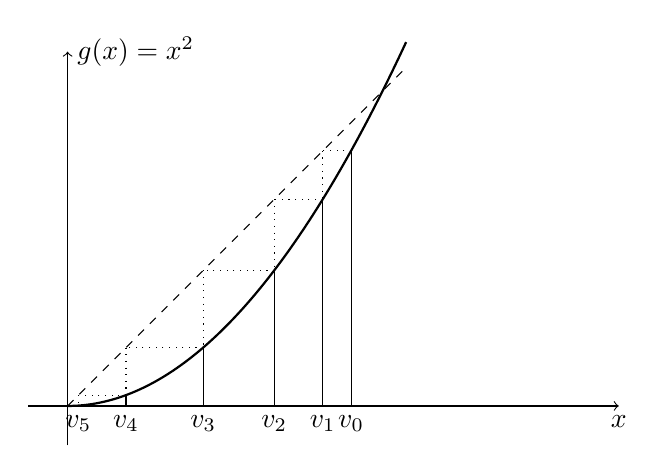
\begin{tikzpicture}
      
      \draw[->] (-0.5, 0) -- (7, 0) node[below] {$x$};
      \draw[->] (0, -0.5) -- (0, 4.5) node[right] {$g(x) = x^2$}; 
        

      \draw[black, dashed] (0, 0) -- (4.3, 4.3);

      \draw[black] (0.9 * 4, 0) node[below] {$v_0$} -- (0.9 * 4, 0.81 * 4);
      \draw[black, dotted] (0.9 * 4, 0.81 * 4) -- (0.81 * 4, 0.81 * 4);
      \draw[black, dotted] (0.81 * 4, 0.81 * 4) -- (0.81 * 4, 0);
      
      \draw[black] (0.81 * 4, 0) node[below] {$v_1$} -- (0.81 * 4, 0.6561 * 4);
      \draw[black, dotted] (0.81 * 4, 0.6561 * 4) -- (0.6561 * 4, 0.6561 * 4);
      \draw[black, dotted] (0.6561 * 4, 0.6561 * 4) -- (0.6561 * 4, 0);
      
      \draw[black] (0.6561 * 4, 0) node[below] {$v_2$} -- (0.6561 * 4, 0.4305 * 4);
      \draw[black, dotted] (0.6561 * 4, 0.4305 * 4) -- (0.4305 * 4, 0.4305 * 4);
      \draw[black, dotted] (0.4305 * 4, 0.4305 * 4) -- (0.4305 * 4, 0);
      
      \draw[black] (0.4305 * 4, 0) node[below] {$v_3$} -- (0.4305 * 4, 0.1853 * 4);
      \draw[black, dotted] (0.4305 * 4, 0.1853 * 4) -- (0.1853 * 4, 0.1853 * 4);
      \draw[black, dotted] (0.1853 * 4, 0.1853 * 4) -- (0.1853 * 4, 0);
      
      \draw[black] (0.1853 * 4, 0) node[below] {$v_4$} -- (0.1853 * 4, 0.0343 * 4);
      \draw[black, dotted] (0.1853 * 4, 0.0343 * 4) -- (0.0343 * 4, 0.0343 * 4);
      \draw[black, dotted] (0.0343 * 4, 0.0343 * 4) -- (0.0343 * 4, 0);
      
      \draw[black] (0.0343 * 4, 0) node[below] {$v_5$} -- (0.0343 * 4, 0);
      
      
      \draw[thick, smooth, domain=0:4.3, samples=100] plot(\x, {(\x/2)^2});

    \end{tikzpicture}
    \caption{Construction des termes de la suite de vérifiant la relation de récurrence $v_{n+1} = v_n^2$ pour le permier terme $v_0 = \frac {9} {10}$. $g: x \mapsto x^2$ est croissante sur $[0, +\infty[$, et l'on remarque effectivement que la suite $v$ est monotone.}
  \end{figure}
\end{question_kholle}

\begin{question_kholle}
  [Montrons que : $ \overset{\circ}{\Q} = \emptyset $]
  {L'intérieur de l'ensemble des rationnels est vide.}
  Par l'absurde, supposons que $\Q$ possède au moins un point intérieur. \\ Fixons $r_0 \in \overset{\circ}{\Q}$. Par définition d'un point intérieur, il existe $\varepsilon \in \R _+ ^* $ : $]r_0 - \varepsilon , \ r_0 + \varepsilon[ \subset \Q$. Or, par densité des irrationnels dans $\R$, il existe $\alpha \in \R \backslash \Q$ : $r_0 - \varepsilon < \alpha < r_0 + \varepsilon$. On en déduit que $\alpha \in ]r_0 - \varepsilon , \ r_0 + \varepsilon[$, or $]r_0 - \varepsilon , \ r_0 + \varepsilon[ \subset \Q$ donc $\alpha \in \Q$ ce qui contredit le choix de $\alpha \in \R \backslash \Q$. Ainsi, $\overset{\circ}{\Q} = \emptyset$
\end{question_kholle}

\begin{question_kholle}
  [Soient $f,g \ : \ \mathcal{D} \to \R$, $\ell \in \R$ et $a \in \overline{\mathcal{D}}$ tels que $|f(x) - \ell| \leq g(x)$ au voisinage de $a$ et $g$ tend vers $0$ en $a$. Alors $f$ tend vers $\ell$ en $a$.]
  {Théorème sans nom version continue au voisinage de $a$}

  On traite le cas $a\in \R$. Par définition de $|f(x) - \ell| \leq g(x)$ au voisinage de $a$,
  \[
    \exists \eta \in \R _+ ^* \ : \ \forall x \in \mathcal{D}, \ |x-a| \leq \eta \ \implies \ |f(x) - \ell| \leq g(x).
  \]
  Fixons un tel $\eta$. \\
  Soit $\omega \in \R_+ ^*$. Appliquons la définition de $\lim_{x \to a} g(x) = 0$ pour $\varepsilon \gets \omega$ :
  \[
    \exists \eta' \in \R_+ ^* \ : \ \forall x \in \mathcal{D}, \ |x-a| \leq \eta' \ \implies \ |g(x)| \leq \omega.
  \]
  Fixons un tel $\eta'$. \\
  Posons $\Omega = \min{ \{\eta,  \eta' \} }$. \\
  Soit $x\in \mathcal{D}$ tel que $|x-a| \leq \Omega$.
  \[
    |f(x) - \ell | \leq g(x) \leq \omega,
  \]
  car la définition de $\Omega$ permet de remplir les conditions des deux propriétés.
\end{question_kholle}
\end{document}
